% Этот шаблон документа разработан в 2017 году
% Владимиром Коротковым (kvamob@mail.ru) 
%  

\documentclass[a4paper,12pt]{article} % добавить leqno в [] для нумерации слева

%% Глобальные Параметры страницы
\usepackage[left=3cm,right=2cm,top=1cm,bottom=2cm,bindingoffset=0cm]{geometry}

%\includeonly{O-41/h_granite.tex}

%\usepackage{fp} 						% Вычисления с плавающей точкой
%\usepackage{siunitx}					% При использовании пакета fp все числа должны иметь decimal delimiter точку
%\sisetup{output-decimal-marker={,}}	% Числа выводятся с запятой в качестве разделителя разрядов: \num{3.2} выводит 3,2 

%%% Работа с русским языком
\usepackage{cmap}					% поиск в PDF
\usepackage{mathtext} 				% русские буквы в формулах
\usepackage[T2A]{fontenc}			% кодировка
\usepackage[utf8]{inputenc}			% кодировка исходного текста
\usepackage[english,russian]{babel}	% локализация и переносы

%%% 
%\usepackage{rotating}				% Поворот текста

%%% Дополнительная работа с математикой
\usepackage{amsmath,amsfonts,amssymb,amsthm,mathtools} % AMS
\usepackage{icomma} % "Умная" запятая: $0,2$ --- число, $0, 2$ --- перечисление
\usepackage{gensymb}	% Градусы
%% Номера формул
%\mathtoolsset{showonlyrefs=true} % Показывать номера только у тех формул, на которые есть \eqref{} в  тексте.

%% Шрифты
\usepackage{euscript}	 % Шрифт Евклид
\usepackage{mathrsfs} % Красивый матшрифт


%% Перенос знаков в формулах (по Львовскому)
% \newcommand*{\hm}[1]{#1\nobreak\discretionary{}
%	{\hbox{$\mathsurround=0pt #1$}}{}}

%%% Работа с картинками
\usepackage{graphicx}  % Для вставки рисунков
%\usepackage[export]{adjustbox}
\graphicspath{{images/}}  % папки с картинками
\setlength\fboxsep{3pt} % Отступ рамки \fbox{} от рисунка
\setlength\fboxrule{0.2pt} % Толщина линий рамки \fbox{}
\usepackage{wrapfig} % Обтекание рисунков и таблиц текстом


%%% Работа с таблицами
\usepackage{array,tabularx,tabulary,booktabs} % Дополнительная работа с таблицами
\usepackage{longtable}  % Длинные таблицы
\usepackage{multirow} % Слияние строк в таблице

%%% Подписи к рисункам и таблицам в русской типографской традиции
\usepackage{caption} 
\DeclareCaptionFormat{GOSTtable}{#2#1\\#3}
\DeclareCaptionLabelSeparator{fill}{\hfill}
\DeclareCaptionLabelSeparator{dot}{. }
\DeclareCaptionLabelFormat{fullparents}{\bothIfFirst{#1}{~}#2}
\captionsetup[table]{
	format=GOSTtable,
	font={footnotesize},
	labelformat=fullparents,
	labelsep=fill,
	labelfont=rm,
%	labelfont=it,
	textfont=bf,
	justification=centering,
	singlelinecheck=false
}
\captionsetup{font=small}
\captionsetup[figure]{
	labelsep=dot, 
%	textfont=it
}
% А можно и так
%\captionsetup{labelsep=period}


%%% Модификация команд, задающих разделы
% Не подавлять отступы у первого абзаца

\makeatletter   % Команда \makeatletter делает символ @ буквой, команда \makeatother возвращает всё на свои места.
% Разрешим отступ у первого абзаца
\renewcommand\section{\@startsection {section}{1}{\parindent}%
	{3.5ex \@plus 1ex \@minus .2ex}{2.3ex \@plus.2ex}%
	{\normalfont\hyphenpenalty=10000\Large\bfseries}}

\renewcommand\subsection{\@startsection {subsection}{1}{\parindent}%
	{3.5ex \@plus 1ex \@minus .2ex}{2.3ex \@plus.2ex}%
	{\normalfont\hyphenpenalty=10000\large\bfseries}}
\makeatother

% После номеров разделов \section ставить точки
\usepackage{secdot}			
% И после \subsection тоже ставить точки
\sectiondot{subsection}		

\usepackage{lastpage} % Узнать, сколько всего страниц в документе.

\usepackage{soulutf8} % Модификаторы начертания

%\usepackage{hyperref}
%\usepackage[usenames,dvipsnames,svgnames,table,rgb]{xcolor}
%\hypersetup{				% Гиперссылки
%	unicode=true,           % русские буквы в раздела PDF
%	pdftitle={Заголовок},   % Заголовок
%	pdfauthor={Автор},      % Автор
%	pdfsubject={Тема},      % Тема
%	pdfcreator={Создатель}, % Создатель
%	pdfproducer={Производитель}, % Производитель
%	pdfkeywords={keyword1} {key2} {key3}, % Ключевые слова
%	colorlinks=true,       	% false: ссылки в рамках; true: цветные ссылки
%	linkcolor=red,          % внутренние ссылки
%	citecolor=green,        % на библиографию
%	filecolor=magenta,      % на файлы
%	urlcolor=cyan           % на URL
%}

\usepackage{multicol} % Несколько колонок

\usepackage{fancyhdr} % Колонтитулы
%\pagestyle{fancy}
%\renewcommand{\headrulewidth}{0mm}  % Толщина линейки, отчеркивающей верхний колонтитул
%\lfoot{Нижний левый}
%\rfoot{Нижний правый}
%\rhead{Верхний правый}
%\chead{Верхний в центре}
%\lhead{Верхний левый}
% \cfoot{Нижний в центре} % По умолчанию здесь номер страницы


%%%%%%%%%%%%%%%%%%%%%%%%%%%%%%%%%%%%%%%%%%%%%%%%%%%%%%%%%%%%%%%%%%%%%%%%%%%%%%%%%%%%%%%%%%%%%%%%%%%%%%%%%
%%% PAYLOAD
%%%%%%%%%%%%%%%%%%%%%%%%%%%%%%%%%%%%%%%%%%%%%%%%%%%%%%%%%%%%%%%%%%%%%%%%%%%%%%%%%%%%%%%%%%%%%%%%%%%%%%%%%

%%% Заголовок
\author{ООО <<Гидросфера>>}\label{company}
\title{ПАСПОРТ РАЗВЕДОЧНО-ЭКСПЛУАТАЦИОННОЙ СКВАЖИНЫ}
\date{\today}
%%%======================================================================================================
\newbool{ShowCadaster}					% Если true, то показывать кадастровый номер

\newcommand{\txtExecutor}{ООО <<Гидросфера>>}	% Исполнитель
\newcommand{\txtYear}{2018}						% Год
\newcommand{\txtNumber}{№ 1р-э}  				% Номер скважины
\newcommand{\txtPump}{<<Напор>>}  				% Марка насоса
\newcommand{\txtOgolovok}{+0,4}					% Высота оголовка
%
\newcommand{\txtAddress}{--Address--} 		% Адрес
\newcommand{\txtHeight}{}					% Абс. отметка устья скважины
\newcommand{\txtCadaster}{--Cadaster--} 	% Кадастровый номер
\booltrue{ShowCadaster}						% Показывать кадастр.номер, иначе закомментировать эту строку
\newcommand{\txtCoords}{000,000 000,000}	% Координаты скважины
\newcommand{\txtDepth}{0.0}					% Глубина скважины
\newcommand{\txtDebit}{0.0}					% Дебит скважины
\newcommand{\txtLevel}{0.0}					% Уровень воды в скважине
\newcommand{\txtHorizDepth}{0.0}			% Глубина залегания водоносного горизонта
%% ../ приуроченных к ...
\newcommand{\txtGeology}{трещиноватым разностям палеозоя}  %%% ПРИУРОЧЕННЫХ К ...
%% ОБСАДКА
\newcommand{\txtCondMaterial}{полиэтиленовая}	% п/э или стальная труба
\newcommand{\txtCondDiam}{160}					% Диаметр кондуктора
\newcommand{\txtCondBtm}{0.0}					% Длина кондуктора
\newcommand{\txtTubeMaterial}{полиэтиленовая}	% п/э или стальная труба
\newcommand{\txtTubeDiam}{128}					% Диаметр трубы
\newcommand{\txtTubeBtm}{0.0}					% Длина трубы
\newcommand{\txtHoleDiam}{132}					% Диаметр открытого ствола
\newcommand{\txtPumpDepth}{0.0}					% Глубина погружения насоса

%% ГЕОЛОГИЧЕСКИЙ РАЗРЕЗ
\newcommand{\txtGeological}{
	%  N   Возр       Грунты                                       от       до    Категория
	1. & Q IV а & Почвенно-растительный слой, кора выветривания & 0    & 0,5       & III \\  \hline
	2. & Mz     & Кора выветривания - суглинки                  & 0,5  & 10,0      & V   \\  \hline
	3. & Pz     & Скальные грунты  трещиноватые                 & 10,0 & \num{\txtDepth} & VIII \\ \hline
%	&  &  &  &  &  \\ 	\hline 
%	&  &  &  &  &  \\ 	\hline 
%	&  &  &  &  &  \\ 	\hline 
}

%% ВЫЧИСЛЯЕМЫЕ ПОЛЯ (Используется пакет fp)
\FPeval\LevelDyn{round(txtLevel + 5, 1)}	% Динамический уровень воды
\FPeval\DebitRel{round(txtDebit / 5, 2)}	% Удельный дебит
\FPeval\DepthWT{round(txtDepth - 2 / 5, 1)}	% Загружение водоподъемной трубы
\FPeval\DepthAT{round(LevelDyn + 1, 1)}		% Загружение воздухопроводной трубы

%% Результаты откачки
\newcommand{\txtPumpResults}{
57,0 & 		% 
\num{\DepthWT} & 		% Загружение водоподъемной трубы
32,0 & 		%
\num{\DepthAT}  &		% Загружение воздухопроводной трубы
\num{\LevelDyn} & 	% Динамический уровень (Уровень + понижение)
\num{5.0}  &		% Понижение уровня 
\num{\txtDebit} & % Дебит
\num{\DebitRel}  &		% Удельный дебит
\num{4.0}  &		% 
ПКС			% 
}			%

%%%%%%%%%%%%%%%%%%%%%%%%%%%%%%%%%%%%%%%%%%%%%%%%%%%%%%%%%%%%%%%%%%%%%%%%%%%%%%%%%%%%%%%%%%%%%%%%%%%%%%%%%

\begin{document} % конец преамбулы, начало документа

\setlength{\extrarowheight}{1mm} % Дополнительный интервал между строками таблиц

%% Титульная страница

\begin{titlepage}
	\begin{center}
		\textbf{\txtExecutor}
		\vspace{5.5cm}
		
		{\LARGE ПАСПОРТ РАЗВЕДОЧНО-ЭКСПЛУАТАЦИОННОЙ СКВАЖИНЫ}
		\vspace{0.25cm}
		
		для хозяйственно-бытового водоснабжения
		
		\bigskip
		
		на участке по адресу:

		\bigskip				
		\underline{\txtAddress}
		
		\bigskip
		\ifbool{ShowCadaster}{Кадастровый номер \txtCadaster}{}
%		\ifblank{\txtCadaster}{}{Кадастровый номер \txtCadaster}

		
		\vfill
	
		\bigskip
		
	\end{center}

	\vfill
	
	\newlength{\ML}
	\settowidth{\ML}{«\underline{\hspace{0.7cm}}» \underline{\hspace{2cm}}}
	\hfill
	\begin{minipage}{1.0\textwidth}
		Директор ООО <<Гидросфера>> к.г.м.н.
		\underline{\hspace{\ML}} А.\,А.~Кашкаров\\
	\end{minipage}%
	
	\bigskip
	
	\vfill
	\begin{center}
		Екатеринбург, \txtYear
	\end{center}			

	\end{titlepage}

%%%%%%%%%%%%%%%%%%%%%%%%%%%%%%%%%%%%%%%%%%%%%%%%%%%%%%%%%%%%%%%%%%%%%%%%%%%%%%%%
%\pagestyle{fancy} % применим колонтитул
%\fancyhead{} % очистим хидер на всякий случай
%\fancyhead[LE,RO]{\thepage} % номер страницы слева сверху на четных и справа на нечетных
%\lhead{\text{Паспорт скважины}}
%\fancyfoot{} % футер будет пустой

	\begin{center}
		\textbf{ПАСПОРТ}

		разведочно-эксплуатационной скважины \txtNumber, cооруженной 

		\txtExecutor, г.Екатеринбург

	\end{center}


	\bigskip
	
	Адрес участка: 

	\underline{\txtAddress}

	\bigskip

	\ifbool{ShowCadaster}{Кадастровый номер: \txtCadaster}{}
%	\ifblank{ShowCadaster}{}{Кадастровый номер: \txtCadaster}

	Координаты скважины: \txtCoords
	
	\ifblank{\txtHeight}{}{Абсолютная отметка устья скважины: \txtHeight}

	\begin{figure}[h]
		\fbox{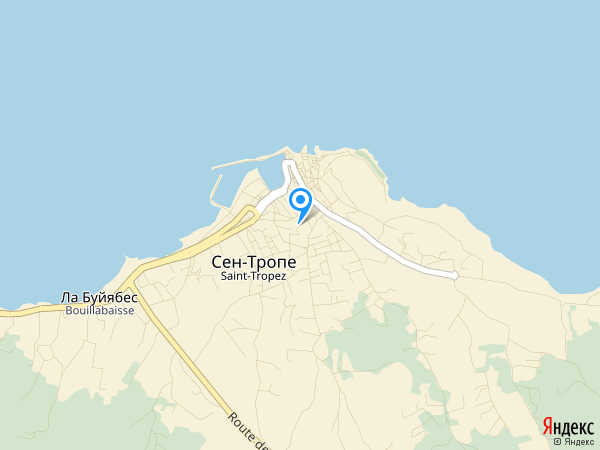
\includegraphics[width=\textwidth]{map.png}}
%		\fbox{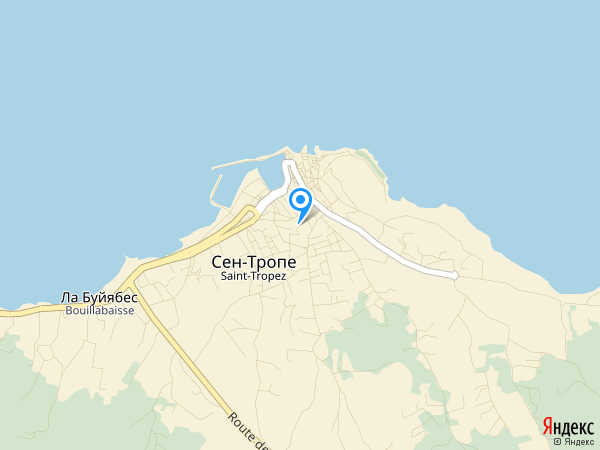
\includegraphics[width=650px]{map.png}}
		\caption{Обзорная карта расположения скважины}
	\end{figure}

    \section{Геолого-технические данные скважины}

    Разведочно-эксплуатационная скважина сооружена \txtExecutor. Имеет общую глубину \num{\txtDepth} \,м.   Бурение производилось вращательно-роторным способом станком УРБ-2-2А.

    \bigskip

%	\settowidth{\ML}{<<\underline{\hspace{0.7cm}}>> \underline{\hspace{2cm}}}
%	\hfill

	\begin{tabular}{@{}ll}
	Бурение начато & << \underline{\hspace{0.7cm}} >> \underline{\hspace{3cm}} \txtYear \,г.\\
	Бурение окончено & << \underline{\hspace{0.7cm}} >> \underline{\hspace{3cm}} \txtYear \,г.\\
	\end{tabular}
	
	\bigskip
	
%	Приемно-сдаточный акт на скважину подписан << >> \txtYear \,г.
	Приемно-сдаточный акт на скважину подписан << \underline{\hspace{0.7cm}} >> \underline{\hspace{3cm}} \txtYear \,г.	
	
	\pagebreak
	
	При бурении скважины пройдены следующие горные породы:
%	\begin{table}[!h]\footnotesize
%	\centering
%	\caption{Геологический разрез по скважине}
%	\begin{tabular}{|p{0.7cm}|p{2cm}|p{7cm}|p{1.5cm}|p{1.5cm}|p{1cm}|}
%		\hline 
%		№№ п.п. & Геологи\-ческий возраст пройденных пород & Описание пройденных пород и характер водоносности & Глубина кровли, м & Глубина подошвы, м & Катего\-рия пород \\ 
%		\hline 
%		\txtGeological  % Геологический разрез см. в преамбуле
%	\end{tabular} 
%	\end{table}

	\begin{table}[!h]\footnotesize
	\centering
	\caption{Геологический разрез по скважине}
	\begin{tabulary}{\textwidth}{|C|C|L|C|C|C|}
	\hline 
	№№ п.п. & Геологический возраст пройденных пород & Описание пройденных пород и характер водоносности & Глубина кровли, м & Глубина подошвы, м & Категория пород \\ 
	\hline 
	\txtGeological  % Геологический разрез см. в преамбуле
	\end{tabulary} 
	\end{table}

	\section{Конструкция скважины}

	Высота оголовка	\underline{\txtOgolovok} м	от поверхности земли. 
	
	\bigskip

	Обсадная колонна:

	диаметром \underline{\txtCondDiam} мм от \underline{\txtOgolovok} м до \underline{\num{\txtCondBtm}}  м  		
	
	диаметром \underline{\txtTubeDiam} мм от \underline{\txtOgolovok} м до \underline{\num{\txtTubeBtm}} м
	
	\bigskip

	Открытый ствол:

	 диаметром \underline{132} мм от \underline{\num{\txtTubeBtm}} до \underline{\num{\txtDepth}} м 
    
    \bigskip
	
	Фильтровая колонна: \underline{нет}
	
%\begin{table}[!h]
%\caption{Устройство скважины}
%\centering
%\begin{tabular}{|c|c|}
%	\hline 
%	№№ & Конструкция: \\ 
%	п.п. & каркас, расположение отверстий, тип, сетка, проволока, диаметр и тд. \\ 
%	\hline 
%	1. & От {\txtOgolovok} до {\num{\txtCondBtm}} м   надфильтровая часть \diameter {\txtCondDiam} мм {\txtCondMaterial} труба \\ 
%	\hline 
%	2. & От {\txtOgolovok} до {\num{\txtTubeBtm}} м   надфильтровая часть \diameter {\txtTubeDiam} мм {\txtTubeMaterial} труба \\ 
%	\hline 
%	3. & От {\num{\txtTubeBtm}} до {\num{\txtDepth}} м   открытый ствол {\diameter} 132 мм \\ 
%	\hline 
%\end{tabular} 
%\end{table}

\begin{table}[!h]
	\caption{Устройство скважины}
	\centering
	\begin{tabularx}{\textwidth}{|c|X|}
		\hline 
		№№ & Конструкция: \\ 
		п.п. & каркас, расположение отверстий, тип, сетка, проволока, диаметр и тд. \\ 
		\hline 
		1. & От {\txtOgolovok} до {\num{\txtCondBtm}} м   надфильтровая часть \diameter {\txtCondDiam} мм {\txtCondMaterial} труба \\ 
		\hline 
		2. & От {\txtOgolovok} до {\num{\txtTubeBtm}} м   надфильтровая часть \diameter {\txtTubeDiam} мм {\txtTubeMaterial} труба \\ 
		\hline 
		3. & От {\num{\txtTubeBtm}} до {\num{\txtDepth}} м   открытый ствол {\diameter} 132 мм \\ 
		\hline 
	\end{tabularx} 
\end{table}


Рабочая часть скважины установлена на основании литологического описания пройденных горных пород и результатов геофизического исследования скважины.

\newpage

Конструкция и глубина сооруженной скважины приведены в следующей таблице:

\bigskip

\begin{table}[!h]
	\caption{Конструкция скважины}
	\centering
\begin{tabular}{rc}
	\hline 
	Глубина в м.: & {\num{\txtDepth}} м \\ 
	\hline 
	Бурение: & Диаметром 165 мм \\ 
	& от 0,0 до {\num{\txtCondBtm}} м \\ 
	& Диаметром {\num{\txtHoleDiam}} мм \\ 
	& от {\num{\txtCondBtm}} до {\num{\txtTubeBtm}} м \\ 
	&  \\ 
	\hline 
	Конструкция: & Бурение от 0,0 до {\num{\txtDepth}} м \\ 
	& Обсадка от {\num{\txtOgolovok}} до {\num{\txtTubeBtm}} м \\ 
	\hline 
	Обсадка: & Диаметром {\txtCondDiam} мм \\ 
	& от {\num{\txtOgolovok}} до {\num{\txtCondBtm}} м \\ 
	& Диаметром {\txtTubeDiam} мм  \\ 
	& От {\num{\txtOgolovok}} до {\num{\txtTubeBtm}} м \\ 
	\hline 
\end{tabular} 
\end{table}

Произведена затрубная гидроизоляция обсадной колонны диаметром \txtTubeDiam \,мм от башмака надфильтровой колонны глухих труб до устья скважины.

Сооруженной скважиной вскрыты водоносные горизонты  подземных вод, приуроченные к \emph{\txtGeology}.

Указанные водоносные горизонты залегают на глубине   \num{\txtHorizDepth} \,– \num{\txtDepth} \,м.

По окончании откачки уровень воды в скважине остановился на глубине  \num{\txtLevel} \,м от поверхности земли.

\section{Результаты откачки}

\begin{table}[!h]
	\caption{Результаты откачки}
	\centering\begin{tabular}{|c|c|c|c|c|c|c|c|c|c|}
	\hline 
	\multicolumn{8}{|c|}{Откачка}&  &  \\ 
	\cline{1-8} 
	\multicolumn{4}{|c|}{Загружение труб, м} &  &  &  &  &  &  \\ 
	\cline{1-4} 
	\multicolumn{2}{|c|}{водоподъемной} & \multicolumn{2}{c|}{воздухопроводной} &  &  &  &  &  & \\ 
	\cline{1-4} 
	\begin{sideways}Диаметр, мм\end{sideways} &
	\begin{sideways}Глубина, м\end{sideways} &
	\begin{sideways}Диаметр, мм\end{sideways} &
	\begin{sideways}Глубина, м\end{sideways} &
	\begin{sideways}Динамический уровень воды, м\end{sideways} &
	\begin{sideways}Понижение уровня, м\end{sideways} &
	\begin{sideways}Дебит, м\textsuperscript{3} /час\end{sideways} &
	\begin{sideways}Удельный дебит, м\textsuperscript{3}/час \end{sideways} &
	\begin{sideways}Продолж-сть откачки, час\end{sideways} &
	\begin{sideways}Марка компрессора\end{sideways} \\ 
	\hline 
%	57,0 & 30,0 & 32,0 & 26,0 & {\txtLevelDynam} & 5,0 & {\txtDebit} & {\txtDebitRel} & 4,0 & ПКС \\ 
	\txtPumpResults \\ 
	\hline 
\end{tabular} 
\end{table}

\subsection{Расчетные данные по результатам откачки}

Водоносный горизонт на рассматриваемой территории залегает на глубине 	{\num{\txtHorizDepth}} - {\num{\txtDepth}}	м, не перекрыт обсадными трубами, представлен открытым стволом, является достаточно защищенным от возможного поверхностного загрязнения.

Учитывая, что скважина \txtNumber \, пробурена для хозяйственно-бытового водоснабжения, организация зоны санитарной охраны на площадке скважины не требуется.

В процессе постоянной эксплуатации скважины рекомендуется периодически производить химический анализ воды для контроля за ее качеством.

\section{Выводы}

В зависимости от фактически полученных результатов откачки и расчетных данных эксплуатация скважины рекомендуется с помощью насоса  \txtPump, при глубине погружения насоса  на \underline{\num{\txtPumpDepth}} \,м от устья скважины с наиболее рациональной производительностью 	{\num{\txtDebit}} м\textsuperscript{3}/час (рекомендуемой \txtExecutor, г. Екатеринбург)

\bigskip

Паспорт составил:

\bigskip

\begin{minipage}{1.0\textwidth}
	Горный инженер-геолог,\\
	кандидат геолого-минералогических наук 
	А.\,А.~Кашкаров
\end{minipage}

\end{document} % конец документа

